\section{Kompilierung von Regelbasen}

Ein naiver Ansatz f�r eine Regelinterpreneter-Implementierung w�re, in jeder Schleife alle Elemente in einer Datenbasis zu vergleichen. Dies w�re langsam und ineffizient. Dieser Prozess kann durch zwei Methoden effizienter gestaltet werden: Begrenzung der zu verarbeitenden Eintr�ge und Begrenzung der zu verarbeitenden Bedingungen.

Um die Anzahl der Eintr�ge pro Schleife zu begrenzen, ist es m�glich, die Ergebnisse eines Vergleichs zu speichern und nur die �nderungen in der Datenbasis auf neue oder entfernte Regeln zu pr�fen. Beim zweiten Ansatz k�nnen �hnliche Tests nur einmal verarbeitet werden, da die Bedingungen f�r Regeln oft nicht disjunkt sind.

\paragraph{Ansatz eines Rate-Algorithmus zur Regelbasenkompilierung}

Regeln werden in ein Netz aus Codest�cken umgewandelt, die Bedingungen darstellen. �hnliche Codest�cke werden kombiniert, um sicherzustellen, dass sie h�chstens einmal verarbeitet werden. Ein Beispiel f�r ein Regelnetz ist in Abbildung~\ref{fig:xps-rule-mesh} dargestellt, und die Kombination dieses Netzes ist in Abbildung~\ref{fig:xps-rule-mesh-combined} zu sehen.

\begin{figure}[H]
    \centering
    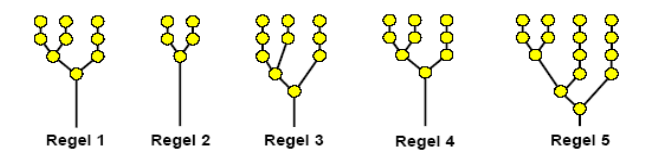
\includegraphics[width=0.8\textwidth]{figures/kap7/rule-mesh.png}
    \caption{Beispiel eines Regelnetzes}
    \label{fig:xps-rule-mesh}
\end{figure}

\begin{figure}[H]
    \centering
    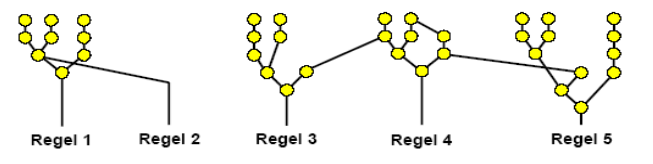
\includegraphics[width=0.8\textwidth]{figures/kap7/combined-rule-mesh.png}
    \caption{Kombinierte Regelnetze}
    \label{fig:xps-rule-mesh-combined}
\end{figure}